\documentclass[12pt,a4paper]{article}

\usepackage{commons/course}


%\hidesolutions



\شروع{نوشتار}
\سربرگ{}{آزمون پایان‌ترم}{28 دی 1398}{}

\vspace*{-2in}
\begin{center}
	به نام او
\end{center}
\vspace*{1.5in}

\section*{سوالات}
امتحان به دو بخش تقسیم می‌شود. 
\\
بخش اول شامل سوالات با پاسخ‌های کوتاه است و بخش دوم شامل 5 سوال تشریحی.

\section*{وقت امتحان}
مدت زمان امتحان 3 ساعت خواهد بود.
\section*{جداول}
جدول های $z$ , $t$ در انتها آمده است. 
\section*{فراموش نکنید:}
\begin{itemize}
	\item با نام و یاد خدا شروع کنید.
	\item هر سوال را در یک برگه جداگانه پاسخ دهید. (در صورت نوشتن چند سوال در یک برگه، فقط یک سوال تصحیح خواهد شد)
	\item بر روی هر برگه اسم و شماره دانشجویی خود را بنویسید.
	\item در صورت داشتن ابهام سوال کنید.
	\item امتحان دارای 7 نمره می‌باشد که 5.1 نمره آن امتیازی است. در صورت کسب بیش از 5.5 نمره، نمره اضافی شما تقسیم بر 2 خواهد شد و به نمره کل اضافه می‌شود.
	
\end{itemize}
\vspace*{1in}
\begin{center}
با آرزوی موفقیت.
\end{center}

\newpage

\section*{کوتاه پاسخ (4 نمره)}
\شروع{ابجد}
\فقره اگر بازه‌ی اطمینان ۹۵‌ درصدی میانگین یک جمعیت $[3, 5]$ باشد، در این صورت درستی یا نادرستی عبارات زیر را مشخص کنید؟ دلیل خود را هم در یک یا دو سطر بیان کنید. (5.1 نمره)
\شروع{فقرات}
\فقره میانگین واقعی  آن جمعیت به احتمال ۹۵ درصد بین ۳ تا ۵ است.
\فقره احتمال آن که میانگین واقعی جمعیت بزرگ‌تر از صفر باشد حداقل ۹۵ درصد است.
\فقره اگر فرایند یافتن بازه‌ی اطمینان ۹۵ درصدی را هزار بار تکرار کنیم حداقل ۹۵۰ بار میانگین واقعی جمعیت در بازه‌ی اطمینان قرار خواهد گرفت.
\پایان{فقرات}

\فقره امید به ریاضی (1 نمره)
\شروع{فقرات}
\فقره فرض کنید متغیرهای تصادفی 
$X_1, X_2, \cdots, X_n$
متغیرهای 
$i.i.d$
هستند. مقدار
$$E[X_1 | X_1 + X_2 + \cdots + X_n = x]$$
که در آن $x$ عدد ثابت است را محاسبه کنید. 
\پایان{فقرات}

\فقره ضریب هم‌بستگی (5.1 نمره)
\\
- درستی یا نادرستی عبارت زیر را با دلیل تعیین کنید.
\شروع{فقرات}
\فقره صفر بودن هم‌بستگی دو متغیر تصادفی \lr{X} و \lr{Y}  دلیلی بر نبودن وابستگی خطی بین  \lr{X} و \lr{Y} نیست.
\پایان{فقرات}

- فرض کنید 3 متغیر تصادفی \lr{A} و \lr{B} و \lr{C}  استاندارد هستند (میانگینشان صفر و واریانسشان یک است). آیا روابط زیر همزمان می‌تواند برقرار باشد؟
\begin{flushleft}
	$corr(A,B)=0.9$ \\
	$corr(B,C)=0.8$ \\
	$corr(A,C)=0.1$
\end{flushleft}



\پایان{ابجد}
\newpage

\مسئله{ (5 نمره)}
ماشینی با احتمال $P_{1}$ عدد 1، با احتمال $P_{2}$ عدد 2 و با احتمال $P_{3}$ عدد 3 را تولید می‌کند. از این ماشین $n$ نمونه گرفته‌ایم که حاوی $x_{1}$ عدد 1 است و $x_{2}$ عدد 2 و $x_{3}$ عدد 3 است. می‌دانیم احتمال تولید چنین نمونه‌هایی طبق توزیع چندجمله‌ای برابر است با:
\\
\begin{flushleft}
	$P(X_{1} = x_{1}, X_{2} = x_{2}, X_{3} = x_{3}) = \frac{n!}{x_{1}!x_{2}!x_{3}!}P_{1}^{x_{1}}P_{2}^{x_{2}}P_{3}^{x_{3}}$
\end{flushleft}
تخمین درست‌نمایی بیشینه را برای $P_{1}$ و $P_{2}$ و $P_{3}$ بدست آورید.

\مسئله{اون‌تر‌نت! (5 نمره)}
همراه ثانی، برای هر کاربر خود عدد تصادفی و مخفی (مثلا $\theta_k$ برای کاربر $k$م) با توزیع یکنواخت بین 0 و 1 تولید می‌کند. این شرکت برای معتاد کردن کاربرانش هر روز به احتمال $\theta_k$ (برای کاربر $k$م)، 2 گیگابایت اینترنت رایگان هدیه می‌دهد. اگر بدانیم در $n$ روز گذشته متین اینترنت رایگان دریافت کرده است، می‌خواهیم احتمال آنکه فردا نیز اینترنت رایگان دریافت کند را بدست آوریم. (دریافت اینترنت در روز $n$اُم را با $X_n$ نشان می‌دهیم.)
\شروع{ابجد}
\فقره با فرض مجهول بودن $\theta$، احتمال این که متین در $n$ روز نخست اینترنت دریافت کرده باشد، چقدر است؟ \\
(به عبارت دیگر $P(X_1=1, \ldots, X_n=1)$ را حساب کنید.)
\فقره توزیع $\theta$ را با فرض این که وی در $n$ روز نخست اینترنت دریافت کرده باشد، بیابید. \\
(به عبارت دیگر $f(\theta=\tau | X_1=1, \ldots, X_n=1)$ را حساب کنید.)
\فقره ثابت کنید $P(X_{n+1}=1 | X_1=1, \ldots, X_n=1)$ برابر است با:
$$\int_0^1 P(X_{n+1}=1 | \theta=\tau) f(\theta=\tau | X_1=1, \ldots, X_n=1) d\tau$$
راهنمایی: با توجه به این که با داشتن $\theta$، دریافت اینترنت در هر روز مستقل خواهد بود داریم:
$$P(X_{n+1}=1 | \theta=\tau) = P(X_{n+1}=1 | \theta=\tau, X_1=1, \ldots, X_n=1)$$
\فقره احتمال دریافت اینترنت در روز $n+1$ را با فرض دریافت اینترنت در $n$ روز قبلی حساب کنید.
\پایان{ابجد}


\مسئله{شکارچی (4 نمره)}
10 شکارچی منتظر پرواز 10 اردک هستند. اردک ها در یک لحظه شروع به پرواز می‌کنند، در آن هنگام هر شکارچی مستقل از دیگران یک اردک را به عنوان هدف انتخاب و به سوی آن شلیک می‌کند. اگر هر شکارچی با احتمال $p$ به هدفش بزند، امید ریاضی تعداد اردک هایی که سالم عبور خواهند کرد را بیابید.

\newpage
\مسئله {کاوه آهنگر (5 نمره)}
کاوه‌، آهنگر سرشناس اصفهان، با معادن استخراج آهن زیادی سر و کله می‌زند. شرط کاوه برای قرار داد بستن با یک معدن، این است که ناخالصی موجود در قطعه آهن عرضه‌شده، برابر با ۷۵ گرم در هر کیلوگرم باشد. او اخیراً شک کرده‌است که یکی از معادنی که قبلاً با آن قرار داد بسته بود، به جای ناخالصی ۷۵ گرم، آهن با ناخالصی ۸۰ گرم به او می‌فروشد. برای آزمایش این فرضیه، به یکی از زیردستانش دستور داده که ناخالصی ۱۰ قطعه آهن یک کیلوگرمی را به عنوان نمونه بررسی کند. اعداد زیر حاصل از بررسی‌های این زیردست هستند:‌

\begin{center}
	\begin{tabular}{|c c c c c c c c c c|} 
		\hline
	76 & 78 & 80 & 70 & 80 & 75 & 73 & 74 & 78 & 76\\ 
		\hline
	\end{tabular}
\end{center}

الف) برای بررسی فرضیه‌ی کاوه، آزمون فرضی بنویسید. سپس در سطح خطای 
$\alpha = 5\%$
و با محاسبه‌ی
$p-value$
این فرضیه را بیازمایید. 

ب) برای آزمونی که در مرحله‌ی قبل طراحی کردید، خطای نوع دو را محاسبه کنید. 

\مسئله {یک پایان تلخ ... (5 نمره)}
در زیر نمرات یک نمونه تصادفی 10 نفره از دانشجویان به عملکرد متین را می‌بینید. عملکرد بسیار بد وی در این ترم به عنوان دستیار آموزشی، باعث شده تا دکتر شریفی نخواهد او را برای دستیاری درس‌های دیگر انتخاب کند اما به دلیل روحیه حساس وی نمی‌خواهد این موضوع را به طور مستقیم به او بگوید. به همین دلیل دکتر این سوال را طرح کرده‌است تا متین با تصحیح ورقه‌های امتحان، خود به عملکرد پایینش پی‌ببرد. 

\begin{center}
	\begin{tabular}{|c|c c c c c c c c c c|} 
		\hline
		نمره عملکرد & 59 & 62 & 59 & 74 & 70 & 61 & 62 & 66 & 62 & 75\\ 
		\hline
	\end{tabular}
\end{center}

\شروع{ابجد}
\فقره یک بازه اطمینان 95 درصدی از میانگین کل نمره عملکرد او بسازید. 
\فقره حال فرض کنيد متوجه شده‌ايم که واريانس نمرات داده شده ۲۵ است. مجدد بازه اطمينان ۹۵ درصدی بسازید و نتيجه را با قسمت قبل مقایسه کنيد.

\پایان{ابجد}



\newpage


\vspace*{1in}
\begin{figure}[h]
	\centering
	
	\textbf{جدول $t$}\par\medskip
	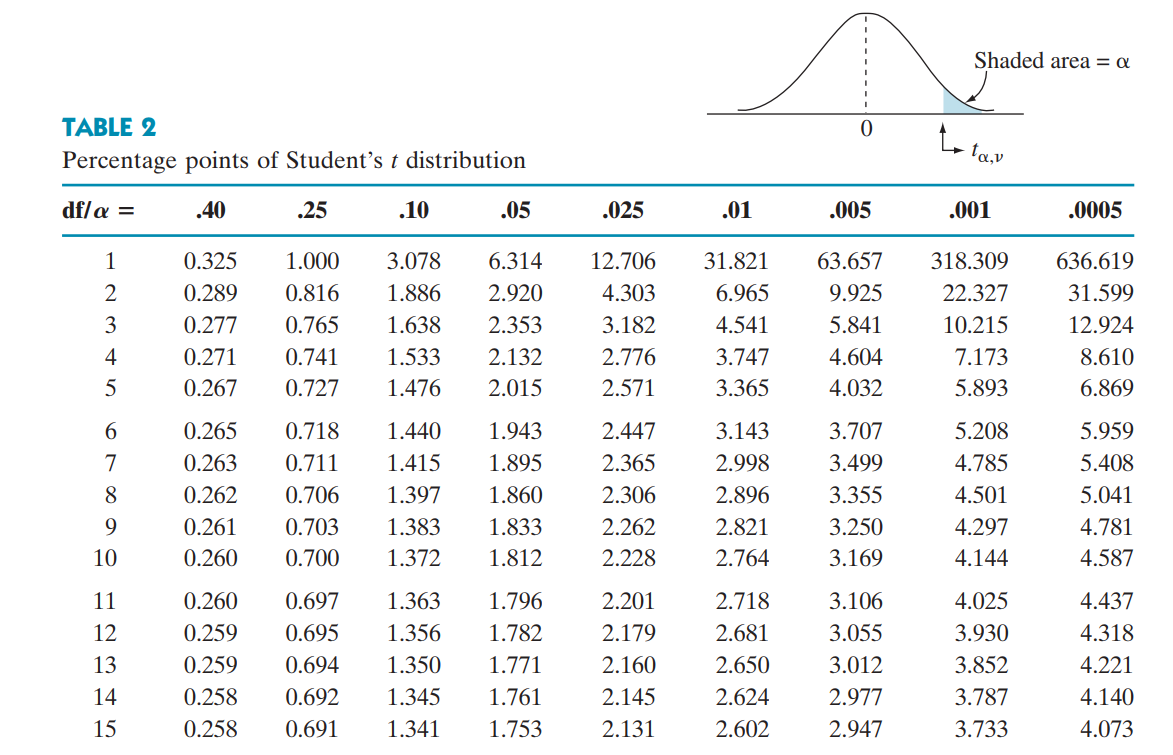
\includegraphics[width=7in,height = 5in]{figs/tStudent}
\end{figure}

\begin{figure}[h]
	\centering
	\textbf{جدول $z$}\par\medskip
	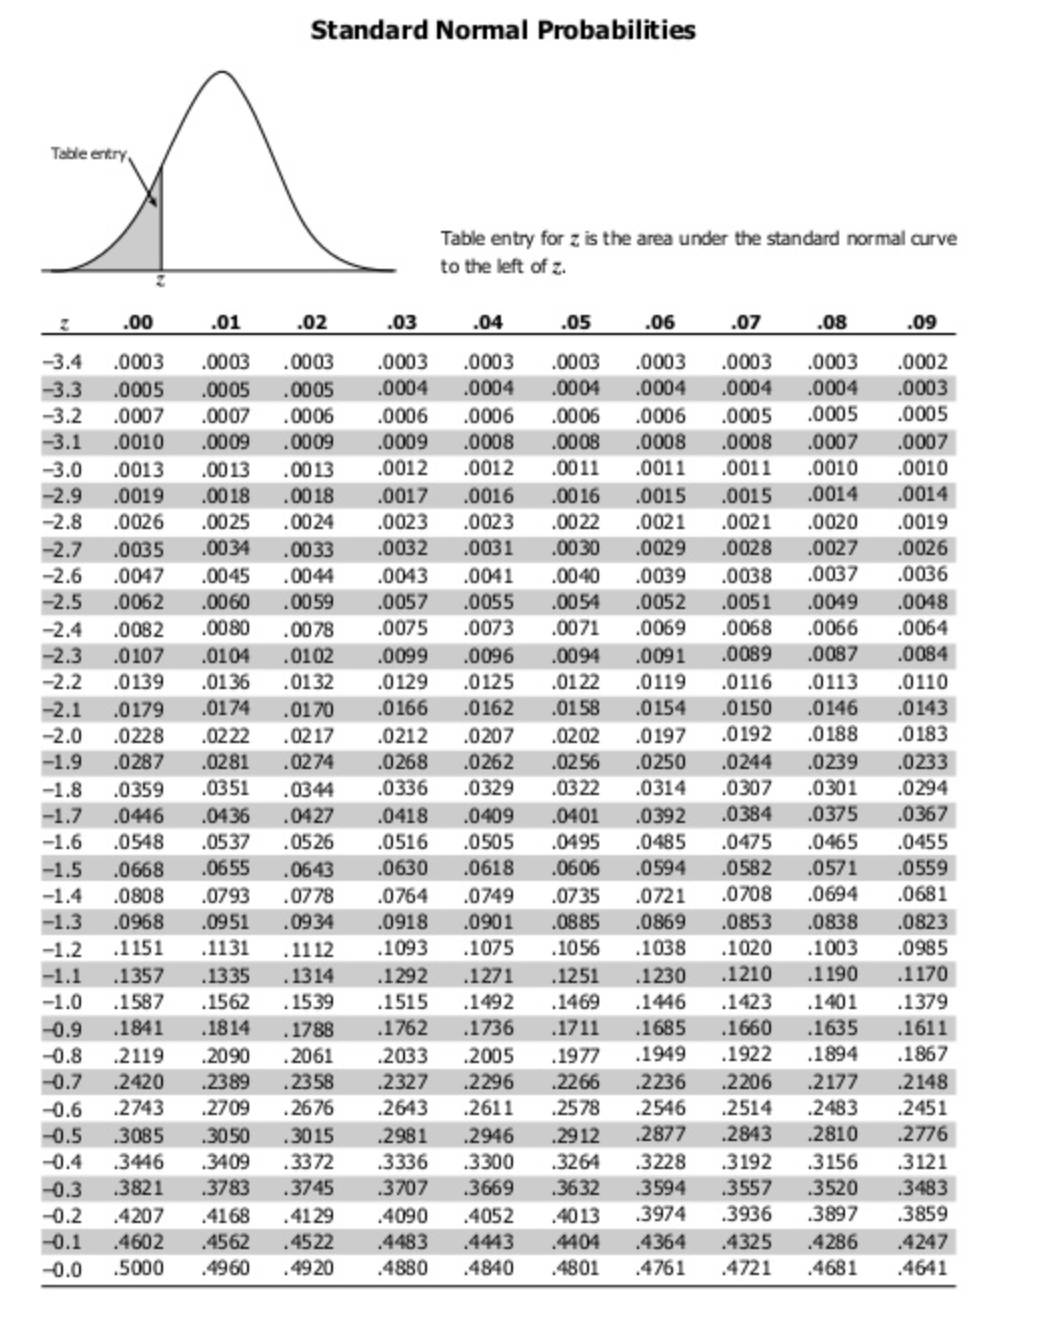
\includegraphics[]{figs/zTable}
\end{figure}
\پایان{نوشتار}
